% !TeX spellcheck = en_GB
\documentclass[12pt]{beamer}

\usetheme[sectionpage=none, subsectionpage=progressbar, progressbar=foot, numbering=fraction]{metropolis}

\makeatletter
\setlength{\metropolis@frametitle@padding}{1.6ex}% <- default 2.2 ex

\setbeamertemplate{footline}{%
  \begin{beamercolorbox}[wd=\textwidth, sep=1.5ex]{footline}% <- default 3ex
    \usebeamerfont{page number in head/foot}%
    \usebeamertemplate*{frame footer}
    \hfill%
    \usebeamertemplate*{frame numbering}
  \end{beamercolorbox}%
}
\makeatother

\AtBeginSubsection
{
  \begin{frame}{Where are we?}
    \tableofcontents[sectionstyle=show/shaded, subsectionstyle=show/shaded/hide]
  \end{frame}
}

\makeatletter
\setbeamertemplate{headline}{
  \begin{beamercolorbox}{upper separation line head}
  \end{beamercolorbox}
  \begin{beamercolorbox}{section in head/foot}
    \vskip2pt\insertsectionnavigationhorizontal{\paperwidth}{}{}\vskip2pt
  \end{beamercolorbox}
  \begin{beamercolorbox}{lower separation line head}
  \end{beamercolorbox}
}
\makeatother
\setbeamercolor{section in head/foot}{fg=normal text.bg, bg=structure.fg}

\setbeamertemplate{itemize items}[square]

\usepackage{menukeys}
\usepackage{minted}
\setminted[bash]{fontsize=\footnotesize, tabsize=2, breaklines}
\setminted[elixir]{fontsize=\footnotesize, tabsize=2, breaklines}
\setminted[erlang]{fontsize=\footnotesize, tabsize=2, breaklines}

\title{Elixir Workshop}
\author{Julius Putra Tanu Setiaji}
\date{13 May 2019}

\begin{document}

\frame[plain]{\titlepage}

\section{First Steps}
\subsection{Erlang}
\begin{frame}{About Erlang}
  \begin{center}
    
\includegraphics[width=0.2\textwidth]{erlang}
  \end{center}
  \begin{itemize}
    \item A development platform for building \textbf{scalable} and \textbf{reliable} systems.
    \item Built in Ericsson\footnote{Ericsson was and is one of the largest telecom infrastructure companies in the world.} in the 1990s
    \item Runs on BEAM (Bj\"{o}rn's Erlang Abstract Machine)\footnote{Similar idea: Java runs on the JVM (Java Virtual Machine)}.
  \end{itemize}
\end{frame}


\begin{frame}{High Availability}
  \begin{itemize}
    \item Fault tolerance
    \item Scalability
    \item Distribution
    \item Responsiveness
    \item Live update
  \end{itemize}
\end{frame}

\begin{frame}{A tribute to Prof. Joe Armstrong}
  \textbf{Prof. Joe Armstrong} was behind the development of Erlang. He passed away recently on 20th April 2019.

  \begin{center}
    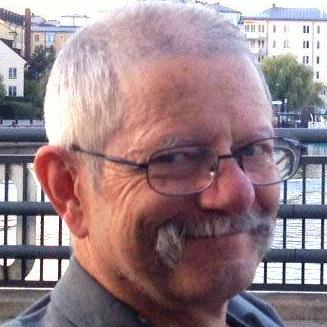
\includegraphics[width=0.4\linewidth]{joearmstrong}
  \end{center}
\end{frame}


\begin{frame}[fragile]{Sample Erlang}
  Based on \textbf{Prolog}: its syntax borrows heavily from it and the first Erlang compiler\footnote{\url{https://www.erlang.se/publications/prac_appl_prolog.ps}} was written in it too.
  \begin{minted}{erlang}
-module(fact).
-export([fac/1]).

fac(0) -> 1;
fac(N) when N > 0, is_integer(N) -> N * fac(N - 1).
  \end{minted}
\end{frame}

\subsection{Elixir}
\begin{frame}{About Elixir}
  \begin{center}
    
\includegraphics[width=0.4\textwidth]{elixir}
  \end{center}
  \begin{itemize}
    \item Targets BEAM, with full Erlang interoperability\footnote{It means that we can use Erlang libraries and tooling}.
    \item Started by Jos\'{e} Valim in 2012 -- he was involved heavily in the Ruby on Rails coreteam before.
    \item Provides almost one-to-one mapping to Erlang constructs but with additions to reduce boilerplate and duplication.
  \end{itemize}
\end{frame}

\begin{frame}[fragile]{Sample Elixir}
  The syntax is heavily borrowed from Ruby.
  \begin{minted}{elixir}
defmodule Fact do
  def fac(0) do
    1
  end

  def fac(n) when n > 0 and is_integer(n) do
    n * fac(n - 1)
  end
end
  \end{minted}
\end{frame}

\begin{frame}{Phoenix Framework}
  \begin{center}
    
\includegraphics[width=0.2\textwidth]{phoenix}
  \end{center}
  \begin{itemize}
    \item Elixir's web framework, just like RoR in Ruby, or Django in Python.
    \item Initially it was heavily based on Ruby on Rails.
    \item Over time, Phoenix has diverged from its Rails roots and developed its own unique ideas.
  \end{itemize}
\end{frame}

\begin{frame}{Ecto}
  \begin{center}
    
\includegraphics[width=0.15\textwidth]{ecto}
  \end{center}
  \begin{itemize}
    \item A database wrapper and language integrated query for Elixir.
    \item Data mapping and validation, with a SQL adapter.
    \item Conceptually, this is the Model in MVC architecture. Similar to ActiveRecord in Ruby on Rails.
  \end{itemize}
\end{frame}

\subsection{Source Academy}
\begin{frame}{Roles of Elixir in Source Academy}
  \begin{itemize}
    \item Source Academy has a separate \textbf{backend} and \textbf{frontend}.
    \item \textbf{Backend} stores data and does the business logic.
    \item \textbf{Frontend} is what the user interacts with and makes requests to the backend.
    \item Phoenix Framework is used to write the Source Academy's backend.
  \end{itemize}
\end{frame}

\begin{frame}{Why Elixir?}
  \begin{itemize}
    \item Elixir has good performance due to BEAM (compared to the alternatives, such as Ruby on Rails, Express on node.js, etc.).
    \item Elixir is a functional language, in line with what CS1101S and SICP taught.
    \item Elixir has more familiar syntax than Erlang.
    \item Good package manager (\texttt{hex} and \texttt{rebar}), which provides ability to use Erlang and Elixir libraries.
  \end{itemize}
\end{frame}

\subsection{Preparing Environment}
\begin{frame}{Steps of Installing Elixir}
  \begin{enumerate}
    \item \textbf{Install Erlang}: I prefer using the native package manager for this (whatever the latest OTP version is)
    \item \textbf{Install Elixir}: I prefer using \texttt{asdf} so I can manage more than 1 version of Elixir at the same time
  \end{enumerate}
\end{frame}

\begin{frame}[fragile]{Installing Erlang}
  On Mac: \url{https://is.gd/install_erlang_mac}

  On Ubuntu: \url{https://is.gd/install_erlang_ubuntu}

  Check if you have a working Erlang/OTP 21 installation:
  \begin{minted}{bash}
$ erl
Erlang/OTP 21 ...

Eshell ...
  \end{minted}
  \begin{minted}{erlang}
> io:fwrite("Hello, world!~n").
Hello, world!
ok
  \end{minted}
\end{frame}

\begin{frame}[fragile]{Installing asdf and Elixir}
  Go to \url{https://asdf-vm.com/}, click on ``Get Started'' and follow the instructions. Afterwards:
  \begin{minted}{bash}
asdf plugin-add elixir
asdf install elixir 1.8.1-otp-21
  \end{minted}

  Check if you have a working Elixir 1.8.1 installation:
  \begin{minted}{bash}
$ iex
Erlang/OTP 21 ...

Interactive Elixir (1.8.1) ...
  \end{minted}
  \begin{minted}{elixir}
iex(1)> IO.puts("Hello, world!")
Hello, world!
:ok
  \end{minted}
\end{frame}

\begin{frame}{Recommended Reading}
  \begin{center}
    \textbf{Elixir in Action by Sasa Juric}

    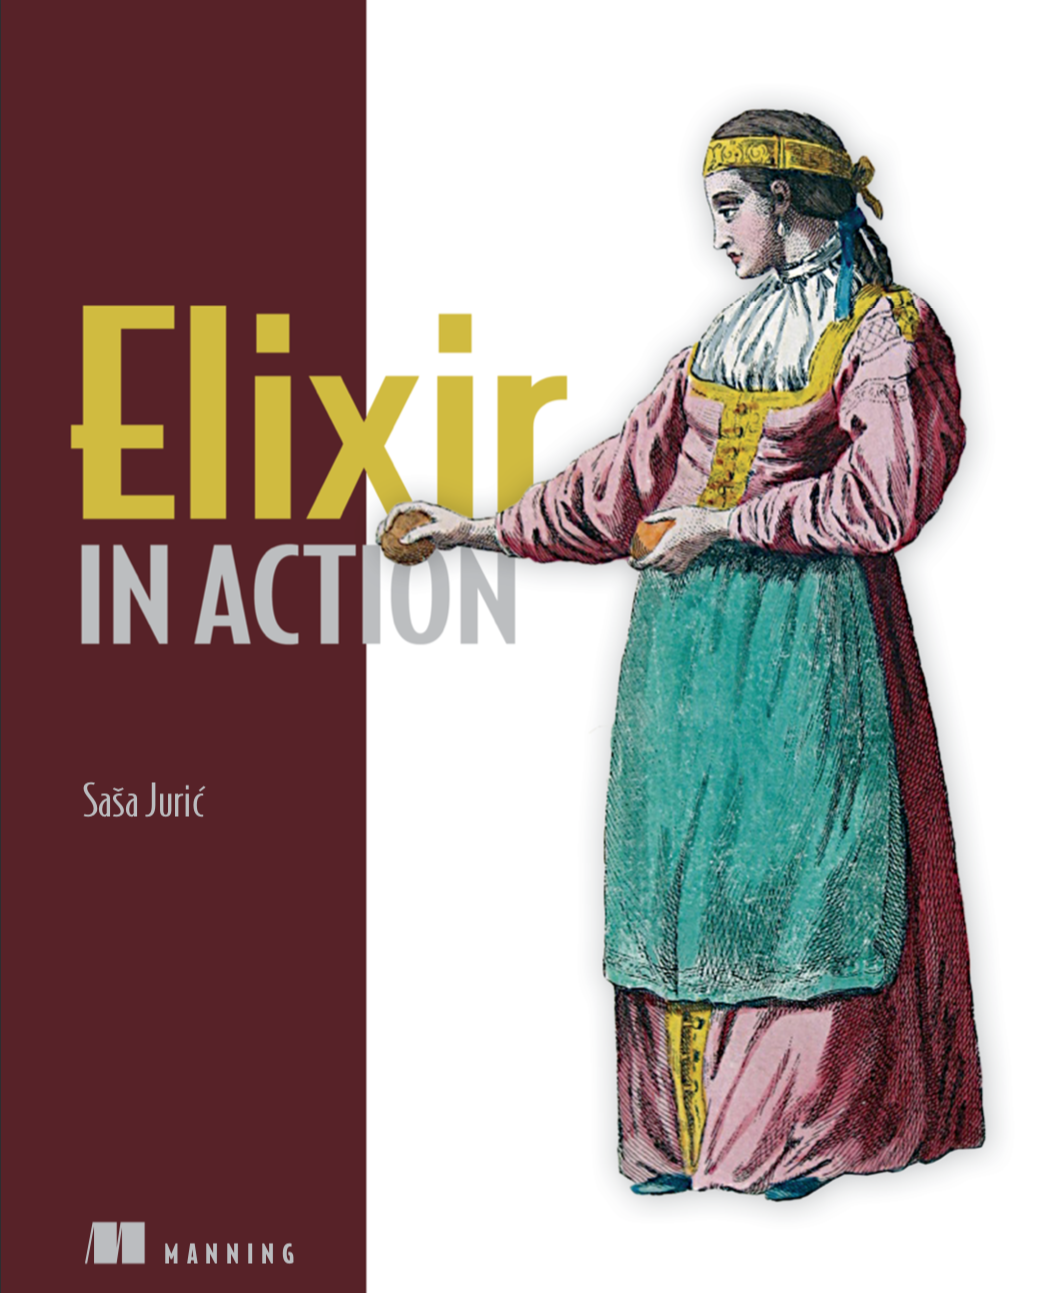
\includegraphics[height=0.5\textheight]{sasajuric}

    The first part would do (first 4 chapters)
  \end{center}
\end{frame}


\section{Building Blocks}
\subsection{The Interactive Shell}
\begin{frame}[fragile]{Elixir Interactive Shell (REPL)}
  \begin{itemize}
    \item You can enter Elixir's REPL\footnote{Read-Evaluate-Print-Loop} by running \mintinline{bash}{iex} from terminal.
    \item \mintinline{elixir}{i}: inspect a value. Example: \mintinline{elixir}{i 5}
    \item \mintinline{elixir}{h}: get help about a command. Examples:
          \begin{minted}{elixir}
h Enum.reduce
h Enum.reduce/2
h Enum.reduce/3
  \end{minted}
    \item Note that in Elixir, everything is an expression and thus will return something.
  \end{itemize}
\end{frame}

\subsection{Variables}
\begin{frame}[fragile]{Variables}
  \begin{itemize}
    \item Elixir is a \textit{dynamic} language, thus there is no explicit type declaration.
    \item In Elixir, mapping a value to a variable is called \textbf{binding}.
    \item To do this, we use the match operator \mintinline{elixir}{=}
    \item Variable names uses snake\_case style.
    \item Example:
          \begin{minted}{elixir}
x = 1
x
y = "a"
y
x = 2
x
  \end{minted}
  \end{itemize}
\end{frame}

\begin{frame}[fragile]{Immutability}
  \begin{itemize}
    \item Elixir is a functional language where everything is immutable.
    \item Re-binding a variable changes the value that a variable is pointing to but never the value itself.
    \item Let's test it with anonymous function:
          \begin{minted}{elixir}
x = 42
foo = fn -> IO.puts(x) end
x = 0
IO.puts(x)
foo.()
        \end{minted}
  \end{itemize}
\end{frame}

\subsection{Organising Your Code}
\begin{frame}{Organising Your Code}
  \begin{itemize}
    \item As a functional language, Elixir relies heavily on functions.
    \item Due to immutable nature of data, typical Elixir program consists of many small functions.
    \item Multiple functions are grouped together into modules.
  \end{itemize}
\end{frame}

\begin{frame}[fragile]{Module and Functions}
  \begin{itemize}
    \item A collection of functions -- similar to namespace in other languages.
    \item Every named function in Elixir must be defined inside a module.
    \item Syntax: \texttt{ModuleName.function\_name(args)}
    \item Module names use CamelCase style. It can also contain the dot character to organise modules hierarchically.
    \item Module definition starts with the \mintinline{elixir}{defmodule} constuct, followed with a \mintinline{elixir}{do}-\mintinline{elixir}{end} block.
    \item Nested module or module whose names contains dot has no special relation -- all modules are independent of one another (for now).
  \end{itemize}
\end{frame}

\begin{frame}{Module and Functions (cont.)}
  \begin{itemize}
    \item Function names use snake\_case style.
    \item Function name conventions: \texttt{?} suffix means the function returns a boolean, \texttt{!} suffis means the function may raise a runtime error.
    \item Function definition starts with the \mintinline{elixir}{def} constuct, followed with a \mintinline{elixir}{do}-\mintinline{elixir}{end} block.
    \item Parantheses can be omitted in definition of 0-arity functions.
    \item No explicit return value -- instead, last expression is the return value.
  \end{itemize}
\end{frame}

\begin{frame}{Modules and Functions (cont.)}
  \begin{itemize}
    \item Default argument is declared using \mintinline{elixir}{\\} -- this creates functions with the same name but different arities
    \item In general, ignored variable are prefixed with underscores.
  \end{itemize}
\end{frame}

\begin{frame}[fragile]{Module and Functions (cont.)}
  Save as \texttt{Geometry.ex}, run as \texttt{iex Geometry.ex}:
  \begin{minted}{elixir}
defmodule Geometry do
  def foo, do: "Hello, world!"

  defmodule Square do
    def area(side \\ 2), do: Geometry.Rectangle.area(side, side)
  end
end

defmodule Geometry.Rectangle do
  def area(length, width) do
    length * width
  end
end
  \end{minted}
\end{frame}

\begin{frame}[fragile]{Module and Functions (cont.)}
  \begin{minted}{elixir}
Geometry.Rectangle.area(2, 5)
Geometry.Square.area(3)
Geometry.foo()
  \end{minted}
\end{frame}

\begin{frame}{Function visibility}
  \begin{itemize}
    \item Functions defined using \mintinline{elixir}{def} is public (exported) and can be used by any module.
    \item To make a function private, define using \mintinline{elixir}{defp} -- private functions can only be invoked inside the module where it is defined.
  \end{itemize}
\end{frame}

\begin{frame}[fragile]{Imports and Aliases}
  \begin{itemize}
    \item \mintinline{elixir}{import} allows calling public functions of a module without prefixing with the module name.
    \item \mintinline{elixir}{alias} allows referencing a module under a different name.
    \item Example:
          \begin{minted}{elixir}
import IO
puts("Hello, world!")
alias Geometry.Square
Square.area(3)
alias Geometry.Square, as: MySquare
MySquare.area(3)
  \end{minted}
  \end{itemize}
\end{frame}

\begin{frame}{Module Attributes}
  Has 3 uses:
  \begin{itemize}
    \item As annotations
    \item As constants at run-time
    \item As temporary storage at compile-time
  \end{itemize}
\end{frame}

\begin{frame}[fragile]{Module Attributes: As annotation}
  Save as \texttt{Foo.ex}, then compile by running \texttt{elixirc Foo.ex}, then run \texttt{iex}
  \begin{minted}{elixir}
defmodule Foo do
  @moduledoc """
  This is the documentation for the Foo module.
  """

  @doc "bar/0 returns the number 5"
  def bar, do: 5
end
  \end{minted}
\end{frame}

\begin{frame}[fragile]{Module Attributes: As constants at run-time}
  \begin{minted}{elixir}
defmodule Geometry.Circle
  @pi 3.14159

  def area(radius), do: @pi * radius * radius
end
  \end{minted}
\end{frame}

\begin{frame}{Comments}
  \begin{itemize}
    \item Comments start with the character \texttt{\#}
    \item Block comments are not supported -- instead prefix each one with \texttt{\#}
  \end{itemize}
\end{frame}

\subsection{Types}
\begin{frame}[fragile]{Identifying functions}
  \begin{itemize}
    \item Functions in Elixir are identified by their name and arity.
    \item The arity of a function describes the number of arguments that the function takes.
    \item Example: \mintinline{elixir}{Enum.reduce/2} identifies a function from the \mintinline{elixir}{Enum} module, function name is \mintinline{elixir}{reduce}, and the arity is 2, while \mintinline{elixir}{Enum.reduce/3} describes the same module, the same function name, but with arity 3.
  \end{itemize}
\end{frame}

\begin{frame}[fragile]{Integer and Float}
  \begin{itemize}
    \item In Elixir, just like in Erlang and Ruby, Integer has arbitrary precision, while float has 64-bit double precision.
    \item Predicate functions: \mintinline{elixir}{is_integer/1} and \mintinline{elixir}{is_float/1}
    \item Note that the \mintinline{elixir}{/} operator always return a float.
    \item To get integer division, use \mintinline{elixir}{div/1} instead.
    \item To get remainder, use \mintinline{elixir}{rem/1}
  \end{itemize}
\end{frame}

\begin{frame}[fragile]{Integer and Float (cont.)}
  \begin{itemize}
    \item Examples:
          \begin{minted}{elixir}
1 + 2
5 * 5
10 / 2
div(10, 2)
rem(10, 3)
rem 10, 3
  \end{minted}
    \item Note that in Elixir, you can drop parantheses when invoking named functions, just like Ruby (generally discouraged)
  \end{itemize}
\end{frame}

\begin{frame}[fragile]{Integer and Float (cont.)}
  \begin{itemize}
    \item Elixir also provides shortcut notation to enter binary, octal, and hexadecimal numbers:
          \begin{minted}{elixir}
0b1010
0o777
0x1F
  \end{minted}
    \item Float requires a dot followed by at least 1 digit.
    \item It also supports \texttt{e} for scientific notation.
    \item You can use \mintinline{elixir}{floor/1}, \mintinline{elixir}{ceil/1}, \mintinline{elixir}{trunc/1}, \mintinline{elixir}{round/1}.
          \begin{minted}{elixir}
1.0
1.0e-10
round(-1.5)
trunc(-1.5)
floor(-1.5)
ceil(-1.5)
  \end{minted}
  \end{itemize}
\end{frame}

\begin{frame}[fragile]{Boolean}
  \begin{itemize}
    \item Either the value \mintinline{elixir}{true} or \mintinline{elixir}{false}
    \item Predicate function: \mintinline{elixir}{is_boolean/1}
    \item Examples:
          \begin{minted}{elixir}
is_boolean(true)
is_boolean(false)
is_boolean(5)
  \end{minted}
  \end{itemize}
\end{frame}

\begin{frame}[fragile]{Atom}
  \begin{itemize}
    \item A constant whose name is its own value. Similar to Symbols in Ruby or Lisp.
    \item Comparison is $O(1)$, while keeping the value named instead of an integer constant.
    \item Syntactically, written with a colon \texttt{:} prefix (like Ruby)
    \item Predicate function: \mintinline{elixir}{is_atom/1}
    \item Example:
          \begin{minted}{elixir}
:test
is_atom(:test)
  \end{minted}
  \end{itemize}
\end{frame}

\begin{frame}[fragile]{Atom (cont.)}
  \begin{itemize}
    \item Note that in Elixir (and Erlang), booleans are implemented as atoms \mintinline{elixir}{:true} and \mintinline{elixir}{:false}, and \mintinline{elixir}{nil} as \mintinline{elixir}{:nil} too.
    \item Module names are atoms too.
    \item You can also specify atom name that contains special characters (such as dot or colon) by delimiting them with double-quotes.
          \begin{minted}{elixir}
is_atom(true)
is_atom(Tuple)
:"Elixir.Tuple"
:"asd:a.sdd"
          \end{minted}
  \end{itemize}
\end{frame}

\begin{frame}[fragile]{String}
  \begin{itemize}
    \item Delimited by double quotes, encoded in UTF-8
    \item Represented internally by binaries (sequence of bytes). Binaries are delimited with \texttt{<<} and \texttt{>>}
    \item Predicate function: \mintinline{elixir}{is_binary/1}
    \item Examples:
          \begin{minted}{elixir}
"Hello, world!"
<<104, 101, 108, 108, 111>>
is_binary("Hi!")
  \end{minted}
    \item Elixir supports string interpolation:
          \begin{minted}{elixir}
"Hello, #{:world}"
  \end{minted}
  \end{itemize}
\end{frame}

\begin{frame}[fragile]{String (cont.)}
  \begin{itemize}
    \item Get number of bytes in a string using \mintinline{elixir}{byte_size/1}
    \item Get length of string using \mintinline{elixir}{String.length/1}
    \item However, they might not be the same as the length of the string due to UTF-8 encoding:
          \begin{minted}{elixir}
byte_size("hellö")
String.length("hellö")
          \end{minted}
    \item \mintinline{elixir}{String} module contains helpful functions to manipulate string:
          \begin{minted}{elixir}
String.upcase("hellö")
        \end{minted}
  \end{itemize}
\end{frame}

\begin{frame}[fragile]{Anonymous functions (lambda)}
  \begin{itemize}
    \item Delimited by keywords \mintinline{elixir}{fn} and \mintinline{elixir}{end}
    \item Functions are first-class citizens: they can be passed as arguments to other functions.
    \item Note that a dot between the variable and parantheses is required to invoke an anonymous function.
    \item Predicate functions: \mintinline{elixir}{is_function/1}, \mintinline{elixir}{is_function/2}
    \item Examples:
          \begin{minted}{elixir}
add = fn a, b -> a + b end
add.(1, 2)
is_function(add)
is_function(add, 2)
is_function(add, 1)
Enum.each('hello', fn x -> IO.puts(x) end)
        \end{minted}
  \end{itemize}
\end{frame}

\begin{frame}[fragile]{The Capture Operator}
  \begin{itemize}
    \item Ampersand \mintinline{elixir}{&} is the capture operator.
    \item It can be used to create anonymous function
    \item Examples:
          \begin{minted}{elixir}
Enum.each('hello', &IO.puts/1)
Enum.each('hello', &IO.puts(&1))
(&IO.puts(&1)) == &IO.puts(&1)
        \end{minted}
  \end{itemize}
\end{frame}

\begin{frame}[fragile]{(Linked) Lists}
  \begin{itemize}
    \item Dynamic, variable-sized collections of data.
    \item The syntax might look like an array, but it actually is a linked list with $O(n)$ complexity for most functions.
    \item It uses Lisp-y list (SICP list): the lists are built from pairs
    \item Syntax for pair: \mintinline{elixir}{[head | tail]}
    \item To get head and tail, use \mintinline{elixir}{hd/1} and \mintinline{elixir}{tl/1} respectively.
    \item Predicate functions: \mintinline{elixir}{is_list/1}
  \end{itemize}
\end{frame}

\begin{frame}[fragile]{(Linked) Lists}
  \begin{itemize}
    \item Examples:
          \begin{minted}{elixir}
[1 | 2]
[1 | [2 | []]]
[1, 2]
is_list([1, 2, 3, 4])
length([1, 2, 3, 4])
        \end{minted}
    \item Concatenate using the \mintinline{elixir}{++/2} operator, subtract using the \mintinline{elixir}{--/2} operator:
          \begin{minted}{elixir}
[1, 2, 3] ++ [4, 5, 6]
[1, true, 2, false, 3, true] -- [true, false]
        \end{minted}
  \end{itemize}
\end{frame}

\begin{frame}[fragile]{(Linked) Lists (cont.)}
  \begin{itemize}
    \item Note that in Erlang, strings are usually represented as charlist (list of characters) instead of binaries.
    \item Charlist is written in Elixir delimited single quote.
    \item Examples:
          \begin{minted}{elixir}
'hello'
[104, 101, 108, 108, 111]
"hello"
<<104, 101, 108, 108, 111>>
'hello' == "hello"
        \end{minted}
  \end{itemize}
\end{frame}

\begin{frame}[fragile]{Tuple}
  \begin{itemize}
    \item Delimited by curly braces.
    \item Group a fixed number of elements, stored contiguously in memory. Thus, most operations are $O(1)$
    \item Examples:
          \begin{minted}{elixir}
tuple = {:ok, "world"}
tuple_size({:ok, "world"})
elem(tuple, 1)
put_elem(tuple, 1, "world")
      \end{minted}
  \end{itemize}
\end{frame}

\begin{frame}{List vs Tuple}
  \begin{itemize}
    \item Appending lists is $O(n)$
    \item Tuples are stored contiguously in memory, thus updating a value in tuple is expensive as a new tuple has to be created.
    \item Tuples are typically used to return more than 1 data from a function: \mintinline{elixir}{{:ok, data}}, \mintinline{elixir}{{:error, :reason}}
    \item Usually, Elixir will guide you to do the right thing: \mintinline{elixir}{elem/1} exists but no built-in equivalent for lists.
    \item When counting elements, in Elixir, \mintinline{elixir}{size} signifies $O(1)$, while \mintinline{elixir}{length} signifies $O(n)$
    \item E.g. \mintinline{elixir}{byte_size/1}, \mintinline{elixir}{tuple_size/1} vs \mintinline{elixir}{length/1}, \mintinline{elixir}{String.length/1}
  \end{itemize}
\end{frame}

\begin{frame}{Operators}
  \begin{itemize}
    \item \textbf{Arithmetic}: \mintinline{elixir}{+}, \mintinline{elixir}{-}, \mintinline{elixir}{*}, \mintinline{elixir}{/}, \mintinline{elixir}{div}, \mintinline{elixir}{rem}
    \item \textbf{List}: \mintinline{elixir}{++}, \mintinline{elixir}{--}
    \item \textbf{Binary (String)}: concatenate \mintinline{elixir}{<>}
    \item \textbf{Boolean}: \mintinline{elixir}{and}, \mintinline{elixir}{or}, \mintinline{elixir}{not}
    \item \textbf{Truthy/Falsey}: \mintinline{elixir}{||} return the first truthy value or the last element, \mintinline{elixir}{&&} return the first falsey value or the last element, \mintinline{elixir}{!} returns \mintinline{elixir}{true} except for \mintinline{elixir}{false} and \mintinline{elixir}{nil}
    \item \textbf{Comparison}: \mintinline{elixir}{==}, \mintinline{elixir}{!=}, \mintinline{elixir}{<=}, \mintinline{elixir}{>=}, \mintinline{elixir}{>}, \mintinline{elixir}{<}, \mintinline{elixir}{===} strict compare integer and float, \mintinline{elixir}{!==}
    \item Different types can be compared with total order\footnote{number < atom < reference < function < port < pid < tuple < map < list < bitstring}.
  \end{itemize}
\end{frame}

\begin{frame}[fragile]{Maps}
  \begin{itemize}
    \item A key-value store, implemented using Hash Array Mapped Trie (HAMT).
    \item Examples:
          \begin{minted}{elixir}
%{a: 1, b: 2}
%{:a => 1, :b => 2}
map = %{"a"=> %{"b" => [true, false, nil]}, 5 => "boo", :z => 100}
map["a"]
map["a"]["b"]
map[:z]
map.z
%{map | 5 => "honhonhon"}
      \end{minted}
  \end{itemize}
\end{frame}

\begin{frame}[fragile]{Keyword List}
  \begin{itemize}
    \item Older way to create a key-value store is having a list of 2-item tuple.
    \item If the first item of the tuple is an atom, then this is a keyword list.
    \item Example:
          \begin{minted}{elixir}
[{:a, 1}, {:b, 2}]
[a: 1, b: 2]
  \end{minted}
    \item Important properties:
          \begin{itemize}
            \item Keys must be atoms
            \item Keys are ordered
            \item Keys can be given more than once.
          \end{itemize}
    \item Beware of the $O(n)$ performance characteristics.
  \end{itemize}
\end{frame}

\begin{frame}[fragile]{Range}
  \begin{itemize}
    \item Represents a range of numbers (like Ruby)
    \item Example:
          \begin{minted}{elixir}
range = 1..2
1 in range
-1 in range
Enum.each(1..3, &IO.puts/1)
    \end{minted}
  \end{itemize}
\end{frame}

\begin{frame}{Macros}
  \begin{itemize}
    \item Advanced feature -- we will not go into much detail.
    \item A very lisp-y feature.
    \item Elixir metaprogramming feature: code that receives AST and manipulates them.
    \item Note that many of the constructs in Elixir are actually implemented as macros on the standard library: \mintinline{elixir}{def}, \mintinline{elixir}{defp}, etc.
  \end{itemize}
\end{frame}

\section{Control Flow}
\subsection{Pattern Matching}
\begin{frame}[fragile]{Pattern Matching}
  \begin{itemize}
    \item One of the most powerful features of functional languages.
    \item Similar to destructuring in Ruby or JavaScript.
    \item Recall the match operator \mintinline{elixir}{=}
    \item So far we have just done simple bindings from the RHS to LHS:
          \begin{minted}{elixir}
x = 1
x
          \end{minted}
  \end{itemize}
\end{frame}

\begin{frame}[fragile]{Pattern Matching (cont.)}
  \begin{itemize}
    \item However, we can also do:
          \begin{minted}{elixir}
1 = x
    \end{minted}
    \item This is because LHS and RHS are both \mintinline{elixir}{1}.
    \item The value in the RHS, namely the value bound to \mintinline{elixir}{x} (i.e. \mintinline{elixir}{1}) is being pattern-matched against the value in the LHS, namely \mintinline{elixir}{1}
    \item However, doing \mintinline{elixir}{2 = x} will result in \mintinline{elixir}{MatchError}
  \end{itemize}
\end{frame}

\begin{frame}[fragile]{Pattern Matching on More Complex Data Types}
  \begin{minted}{elixir}
{name, age} = {"Bob", 25}
{_, {hour, _, _}} = :calendar.local_time()
# Mimicking Prolog's unification. Suck it Haskell!
{amount, amount, amount} = {127, 127, 127}
{amount, amount, amount} = {127, 127, 1}

[first, second, third] = [1, 2, 3]
[head | tail] = [1, 2, 3]

%{name: name, age: age} = %{name: "Bob", age: 25}
%{age: age} = %{name: "Bob", age: 25}

"Hello" <> rest = "Hello, world!"
 \end{minted}
\end{frame}

\begin{frame}[fragile]{Pin Operator \mintinline{elixir}{^}}
  \begin{itemize}
    \item Variables in Elixir can be rebound.
    \item To pattern match against an existing variable's value rather rebinding, use the pin operator \mintinline{elixir}{^}:
          \begin{minted}{elixir}
 x = 1
 ^x = 2
 \end{minted}
  \end{itemize}
\end{frame}

\subsection{Conditionals}
\begin{frame}[fragile]{Pattern Matching on Function Arguments and Multi-clausal Functions}
  In functional languages, you can pattern match on function arguments too, and provide multiple clauses!
  \begin{minted}{elixir}
defmodule Fact do
  def fac(0), do: 1
  def fac(n), do: n * fac(n - 1)
end
 \end{minted}
  For a function, each clause will be attempted based on the order of definition.
\end{frame}

\begin{frame}[fragile]{Function Guards}
  \begin{itemize}
    \item For a factorial function, only non-negative integers are valid input.
    \item Using predicate functions and simple comparison expressions, we can provide constraints more than just the pattern match on each function clause:
          \begin{minted}{elixir}
defmodule Fact do
  def fac(0) do: 1
  def fac(n) when is_integer(n) and n > 0, do: n * fac(n - 1)
end
 \end{minted}
  \end{itemize}
\end{frame}

\begin{frame}{Function Guards (cont.)}
  \begin{itemize}
    \item The set of operators and functions that can be called is very limited, the full list is at \url{https://hexdocs.pm/elixir/guards.html}
    \item Note that error raised in the guard expression will simply result in match failure, and Elixir will move on to the next clause, e.g. applying \mintinline{elixir}{length/1} on a non-list.
  \end{itemize}
\end{frame}

\begin{frame}[fragile]{Multi-clausal lambdas}
  Anonymous functions (lambdas) may also consist of multiple clauses:
  \begin{minted}{elixir}
test_num = fn
  0 -> :zero
  x when is_number(x) and x < 0 -> :negative
  x when is_number(x) and x > 0 -> :positive
end
Enum.map(-2..2, test_num)
 \end{minted}
\end{frame}

\begin{frame}[fragile]{case}
  \begin{itemize}
    \item \mintinline{elixir}{case} allows us to compare a value against many patterns until we find a matching one.
    \item Guards can be used also.
    \item If none of the clauses match, \mintinline{elixir}{CaseClauseError} is raised.
    \item Example:
          \begin{minted}{elixir}
 case {1, 2, 3} do
   {4, 5, 6} -> :no_match
   {1, x, 3} when x > 0 -> :match
   _ -> :match_anything
 end
 x
 \end{minted}
  \end{itemize}
\end{frame}

\begin{frame}[fragile]{case (cont.)}
  In fact, we can reimplement our factorial function using \mintinline{elixir}{case}:
  \begin{minted}{elixir}
defmodule Fact do
  def fac(n) do
    case n do
      0 ->
        1

      x when is_integer(x) and x > 0 ->
        n * fac(n - 1)
    end
  end
end
 \end{minted}
\end{frame}

\begin{frame}[fragile]{cond}
  \begin{itemize}
    \item Used to check for different conditions and find the first clause that is truthy.
    \item Similar to if-else if-else clauses in imperative languages.
    \item Note that idiomatic Elixir uses \mintinline{elixir}{cond} very sparingly.
    \item Example:
          \begin{minted}{elixir}
cond do
  2 + 2 == 5 -> :never_true
  1 + 1 == 2 -> :should_match_this
  true -> :will_match_this_if_all_fail
end
  \end{minted}
  \end{itemize}
\end{frame}

\begin{frame}[fragile]{\mintinline{elixir}{if} and \mintinline{elixir}{unless}}
  \begin{itemize}
    \item To check for only 1 condition, Elixir provides \mintinline{elixir}{if} and \mintinline{elixir}{unless} (if not). They are implemented as macros.
    \item If no block is specified, an implicit \mintinline{elixir}{nil} is returned.
    \item Example:
          \begin{minted}{elixir}
if nil do
  "This won't be seen"
else
  "This will"
end

unless true do
  "This will never be seen"
end
  \end{minted}
  \end{itemize}
\end{frame}

\subsection{Recursion}
\begin{frame}[fragile]{Our Old Friend Recursion!}
  \begin{minted}{elixir}
defmodule Fact do
  def fac(0), do: 1
  def fac(n) when is_integer(n) and n > 0, do: n * fac(n - 1)
end
  \end{minted}
\end{frame}

\begin{frame}[fragile]{And Tail Call Recursions!}
  \begin{minted}{elixir}
defmodule Fact do
  def fac(n, acc \\ 1) when is_integer(n) and is_integer(acc) and acc > 0 do
    case n do
      0 -> acc
      n when n > 0 -> fac(n - 1, acc * n)
    end
  end
end
  \end{minted}
\end{frame}

\subsection{Enumerable}
\begin{frame}[fragile]{Enumerable}
  \begin{itemize}
    \item Elixir provides the concept of enumerables and the \mintinline{elixir}{Enum} module (\url{https://hexdocs.pm/elixir/Enum.html}) to work with them using higher order functions.
    \item Example:
          \begin{minted}{elixir}
# Allow us to use macros in Integer module
require Integer
Enum.reduce(Enum.filter(Enum.map(1..100_000, &(&1 * 3)), &Integer.is_even/1), 0, &+/2)
Enum.sum(Enum.filter(Enum.map(1..100_000, &(&1 * 3)), &Integer.is_even/1))
  \end{minted}
  \end{itemize}
\end{frame}

\begin{frame}[fragile]{The Pipe Operator}
  \begin{itemize}
    \item In my opinion, the best feature that Elixir has!
    \item The pipe operator \mintinline{elixir}{|>} takes the output from the left side and passes it as the first argument to the function call on the right side.
    \item Similar to Unix shell \mintinline{bash}{|} operator.
    \item Clear pipeline of transformation of data.
    \item Example:
          \begin{minted}{elixir}
require Integer
1..100_000
|> Enum.map(&(&1 * 3))
|> Enum.filter(&Integer.is_even/1)
|> Enum.sum()
  \end{minted}
  \end{itemize}
\end{frame}

\subsection{Streams}
\begin{frame}[fragile]{Streams}
  \begin{itemize}
    \item Enumerables are eager. Elixir provides a lazy alternative: the \mintinline{elixir}{Stream} module (\url{https://hexdocs.pm/elixir/Stream.html})
    \item They are composable too.
    \item Examples:
          \begin{minted}{elixir}
stream = Stream.cycle([1, 2, 3])
stream |> Stream.take(4) |> Enum.to_list()
require Integer
1..100_000 |> Stream.map(&(&1 * 3)) |> Stream.filter(&Integer.is_odd/1)
  \end{minted}
  \end{itemize}
\end{frame}

\subsection{Comprehension}
\begin{frame}[fragile]{Comprehension}
  \begin{itemize}
    \item Similar concept to Python's list comprehension, but on steroids (with pattern matching)
    \item Example:
          \begin{minted}{elixir}
values = [good: 1, good: "a", bad: 3, good: 4]
for {:good, n} when is_number(n) <- values, do: n * n
  \end{minted}
    \item Besides pattern matching and guards, filter expression can be used too:
          \begin{minted}{elixir}
multiple_of_3? = fn n -> rem(n, 3) == 0 end
for n <- 0..5, multiple_of_3?.(n), do: n * n
  \end{minted}
  \end{itemize}
\end{frame}

\begin{frame}[fragile]{Comprehension (cont.)}
  \begin{itemize}
    \item Comprehensions also allow multiple generators and filters:
          \begin{minted}{elixir}
dirs = ['/tmp/', '/usr/lib']
for dir <- dirs,
    file <- File.ls!(dir),
    path = Path.join(dir, file),
    File.regular?(path) do
  File.stat!(path).size
end
  \end{minted}
  \end{itemize}
\end{frame}

\begin{frame}[fragile]{Comprehension (cont.)}
  \begin{itemize}
    \item Using \mintinline{elixir}{:into}, result of a comprehension can be inserted into different data structures:
          \begin{minted}{elixir}
for <<c <- " hello world ">>, c != ?\s, into: "", do: <<c>>

for {key, val} <- %{"a" => 1, "b" => 2}, into: %{}, do: {key, val * val}
  \end{minted}
  \end{itemize}
\end{frame}

\begin{frame}[fragile]{Comprehension (cont.)}
  Using comprehension, we can even implement quicksort!
  \begin{minted}{elixir}
defmodule Sort do
  def qsort([]) do
    []
  end

  def qsort([x | xs]) do
    qsort(for a when a < x <- xs, do: a) ++ [x] ++ qsort(for a when a >= x <- xs, do: a)
  end
end
  \end{minted}
\end{frame}

\section{Other Useful Features}
\subsection{Struct}
\begin{frame}[fragile]{Struct}
  \begin{itemize}
    \item Extensions built on top of maps that provide compile-time checks and default values.
    \item Defined using \mintinline{elixir}{defstruct} construct:
          \begin{minted}{elixir}
defmodule User do
  defstruct name: "John", age: 27
end

%User{}
%User{oops: :field}
jane = %User{age: 10, name: "Jane"}
%{jane | age: 11}
%{name: name} = jane
name
jane.name
is_map(jane)
  \end{minted}
  \end{itemize}
\end{frame}

\begin{frame}{Struct (cont.)}
  \begin{itemize}
    \item In Phoenix Framework, ecto data are abstracted as a struct.
    \item However, ecto provides us with special constructs (using macros) to specify the struct fields, so typically in using the Phoenix Framework, we rarely need to use \mintinline{elixir}{defstruct}
    \item However, other syntaxes such as initialising a struct, updating a field, etc. are still used extensively.
  \end{itemize}
\end{frame}

\subsection{Polymorphism with Protocols}
\begin{frame}[fragile]{Protocol}
  \begin{itemize}
    \item A mechanism in Elixir to achieve polymorphism.
    \item Dispatching on a protocol is available to any data type as long as it implements the protocol.
    \item Defined using \mintinline{elixir}{defprotocol}
    \item Example:
          \begin{minted}{elixir}
defprotocol Size do
  @doc "Calculates the size (not the length!) of a data structure"
  def size(data)
end
  \end{minted}
    \item the \texttt{Size} protocol expects a 1-arity function called \texttt{size} to be implemented.
  \end{itemize}
\end{frame}

\begin{frame}[fragile]{Protocol (cont.)}
  \begin{itemize}
    \item Implementation is defined using \mintinline{elixir}{defimpl}
          \begin{minted}{elixir}
defimpl Size, for: BitString do
  def size(string), do: byte_size(string)
end

defimpl Size, for: Map do
  def size(map), do: map_size(map)
end

defimpl Size, for: Tuple do
  def size(tuple), do: tuple_size(tuple)
end
  \end{minted}
  \end{itemize}
\end{frame}

\begin{frame}[fragile]{Protocol (cont.)}
  \begin{itemize}
    \item With the protocol and implementation defined, we can start using it.
    \item Passing a data type that doesn't implement the protocol raises \mintinline{elixir}{Protocol.UndefinedError}.
          \begin{minted}{elixir}
Size.size("foo")
Size.size({:ok, "Hello"})
Size.size(%{label: "some label"})
Size.size([1, 2, 3])
Size.size(%User{})
  \end{minted}
    \item Protocols can be implemented for all Elixir data types, as well as user-defined structs:
          \begin{minted}{elixir}
defimpl Size, for: User do
  def size(_user), do: 2
end
  \end{minted}
  \end{itemize}
\end{frame}

\begin{frame}{Protocol (cont.)}
  \begin{itemize}
    \item Elixir ships with some built-in protocols.
    \item For example, \mintinline{elixir}{Enum} module provides functions that work with any data structure that implements the \mintinline{elixir}{Enumerable} protocol.
  \end{itemize}
\end{frame}

\subsection{Sigil}
\begin{frame}{Sigils}
  \begin{itemize}
    \item Like Perl and Ruby, Elixir has sigils too.
    \item Strings are delimited by double-quotes. Double-quotes inside a string must be escaped.
    \item These kinds of representation problems is what sigils try to solve.
    \item Unlike Perl and Ruby, Elixir only allows a limited set of delimiters: \texttt{//, ||, "", '', (), [], {}, <>}
  \end{itemize}
\end{frame}

\begin{frame}[fragile]{String, Charlist, Word List Sigils}
  \begin{itemize}
    \item \texttt{~s} sigil is used to generate string
    \item \texttt{~c} sigil is used to generate char lists
    \item \texttt{~w} sigil is used to generate lists of words (separated by whitespace).
    \item The \texttt{~w} sigil also accepts the \texttt{c}, \texttt{s}, \texttt{a} modifiers (for char lists, strings and atoms respectively) to specify the data type of the elements of the resulting list.
  \end{itemize}
\end{frame}

\begin{frame}[fragile]{String, Charlist, Word List Sigils (cont.)}
  \begin{minted}{elixir}
~s(a string with "double quotes")
~c|a charlist with 'single quotes' and (parantheses)|
~w(foo bar bat)
~w(ok error)a
  \end{minted}
\end{frame}

\begin{frame}[fragile]{Regular Expressions}
  \begin{itemize}
    \item Elixir provides Perl-compatible regexes, as implemented by the PCRE library.
    \item \textbf{A word of caution}: ``Some people, when confronted with a problem, think I know, I'll use regular expressions. Now they have two problems'' (Zawinski, 1997)\footnote{There is also an interesting read at \url{https://blog.codinghorror.com/regular-expressions-now-you-have-two-problems/}}
    \item There exists a \mintinline{elixir}{Regex} module in Elixir, as well as the regex match operator \mintinline{elixir}{=~}, and the \texttt{~r} sigil to specify precompiled regex.
  \end{itemize}
\end{frame}

\begin{frame}[fragile]{Regular Expressions}
  \begin{minted}{elixir}
regex = ~r/foo|bar/
"foo" =~ regex
"bar" =~ regex
"bat" =~ regex
  \end{minted}
\end{frame}

\subsection{Typespec}
\begin{frame}{Typespec}
  \begin{itemize}
    \item One advantage of using Elixir is that we can use tooling for Erlang, a 30 years old language.
    \item This includes type specs, a system of notating types in Erlang/Elixir.
    \item The Elixir compiler doesn't do type check, but one can use the \texttt{dialyzer} tool to perform type check.
    \item Owing to its age, \texttt{dialyzer} is more mature than, say, \texttt{mypy}, especially in terms of type inference\footnote{More information on Erlang type inference in \url{https://it.uu.se/research/group/hipe/papers/succ_types.pdf}}
  \end{itemize}
\end{frame}

\begin{frame}{Typespec (cont.)}
  \begin{itemize}
    \item Not compulsory, but being able to read type spec helps a lot in reading documentation.
    \item Some code that I wrote in Source Academy have type specs.
    \item In source code, typically notated using module attribute \mintinline{elixir}{@spec}
    \item More information in \url{https://hexdocs.pm/elixir/typespecs.html}
  \end{itemize}
\end{frame}

\section{Source Academy Backend: Cadet}
\subsection{Structure}
\begin{frame}{Structure}
  \begin{itemize}
    \item Phoenix Framework:
          \begin{itemize}
            \item Router
            \item Plugs
          \end{itemize}
    \item MVC
          \begin{itemize}
            \item Model
                  \begin{itemize}
                    \item Contexts: inside \texttt{lib/cadet/}
                    \item Migrations: inside \texttt{priv/repo/migrations/}
                    \item Seeds: inside \texttt{priv/repo/seeds.exs}
                  \end{itemize}
            \item View: \texttt{lib/cadet\_web/views/} -- renders json
            \item Controller: inside \texttt{lib/cadet\_web/controllers/}
          \end{itemize}
  \end{itemize}
\end{frame}

\begin{frame}{Structure (Cont.)}
  \begin{itemize}
    \item Jobs: inside \texttt{lib/cadet/jobs/}
          \begin{itemize}
            \item Updater, XML Parser
            \item Autograder
          \end{itemize}
    \item Mix tasks for convenience: inside \texttt{lib/mix/tasks/}
    \item Config files: inside \texttt{config/}
    \item Tests: 98\% test coverage. Every feature are tested.
  \end{itemize}
\end{frame}


\end{document}
